\documentclass[12pt, a4paper]{article}
\usepackage[utf8]{inputenc}
\usepackage[T1]{fontenc}
\usepackage[magyar]{babel}
\usepackage{amsmath, amssymb}
\usepackage{xcolor}
\usepackage{tikz}
\usepackage{geometry}
\geometry{a4paper, margin=2.5cm}

% Új szín definiálása a megadott követelmények alapján
\definecolor{bvred}{rgb}{0.8, 0.0, 0.0}

% Új parancs a fontos részek kiemelésére
\newcommand{\textbfr}[1]{\textbf{\textcolor{bvred}{#1}}}

\begin{document}

\title{\textbfr{Kúpszeletek}}
\author{Készítette:\\Varga Dávid}
\date{}
\maketitle

\section*{Bevezetés: A kúpszeletek térbeli származtatása}

A geometria történetének egyik legszebb és leginkább vizuális témaköre a síkidomok térbeli származtatása. Képzeljünk el egy térbeli egyenest (tengely), és egy ezt metsző, vele $\alpha$ szöget bezáró másik egyenest (alkotó). Ha az alkotót megforgatjuk a tengely körül, egy végtelen, mindkét irányban nyitott \textbfr{kettős kúpfelületet} kapunk. 

Amikor ezt a felületet egy síkkal elmetszünk, a metszetként kapott görbéket összefoglaló néven \textbfr{kúpszeleteknek} nevezzük. A metsző sík és a kúp tengelye által bezárt $\beta$ dőlésszögtől függően négy alapvető esetet (egy speciális és három általános) különböztetünk meg. Az alábbi ábra ezt a négy esetet szemlélteti:



Ezek a görbék nem csupán a tiszta matematikában játszanak kulcsszerepet, hanem a fizikában is: a bolygók pályája a Nap körül ellipszis, a ferdén elhajított test parabolapályán mozog, az alfa-részecskék pedig hiperbolapályán szóródnak az atommagokon. Lássuk a görbék precíz, síkgeometriai származtatását!

\section*{1. A parabola}

A parabola a legegyszerűbb, egyetlen fókuszponttal rendelkező kúpszelet, amelyhez egy kitüntetett egyenes is tartozik.

\textbf{Definíció.} \textit{A sík azon pontjainak halmazát, amelyek egy adott egyenestől (vezéregyenes vagy direktrix) és egy rajta kívül fekvő adott ponttól (fókuszpont) egyenlő távolságra vannak, \textcolor{bvred}{parabolának} nevezzük.}

\subsection*{A parabola egyenletének levezetése}

Vegyünk fel egy derékszögű koordináta-rendszert úgy, hogy a parabola tengelypontja (csúcsa) az origóba essen, szimmetriatengelye pedig az $y$-tengely legyen. Legyen a fókuszpont távolsága az origótól $\frac{p}{2}$, ahol a $p$ paraméter a fókusz és a vezéregyenes távolsága. Ekkor a fókuszpont koordinátái $F\left(0, \frac{p}{2}\right)$, a vezéregyenes egyenlete pedig $y = -\frac{p}{2}$.

Legyen $P(x,y)$ a parabola egy tetszőleges pontja. A definíció értelmében a $P$ pont távolsága az $F$ ponttól megegyezik a vezéregyenestől mért távolságával ($d$). A két pont távolságára vonatkozó képlet alapján:
\[ \overline{PF} = \sqrt{x^2 + \left(y - \frac{p}{2}\right)^2} \]
A pont és a vízszintes vezéregyenes távolsága:
\[ d = \left| y - \left(-\frac{p}{2}\right) \right| = \left| y + \frac{p}{2} \right| \]
A definíció miatt a két távolság egyenlő:
\[ \sqrt{x^2 + \left(y - \frac{p}{2}\right)^2} = y + \frac{p}{2} \]
Mindkét oldalt négyzetre emelve kapjuk:
\[ x^2 + y^2 - py + \frac{p^2}{4} = y^2 + py + \frac{p^2}{4} \]
Az azonos tagok egyszerűsítése és átrendezés után megkapjuk a parabola \textbfr{tengelyponti egyenletét}:
\[ x^2 = 2py \]
Itt a $p$ érték a parabola paramétere, amely meghatározza annak nyitottságát.

\subsection*{Példák a parabola alkalmazására}
\begin{itemize}
    \item \textbf{Fényszórók és parabolaantennák:} A parabola forgatásával kapott paraboloid belső felülete a fókuszpontba helyezett forrás sugarait (fény vagy rádióhullám) párhuzamos nyalábban veri vissza.
    \item \textbf{Ballisztika:} Ha egy testet vízszintes sebességgel elhajítunk, pályájának egyenlete $y = -\frac{g}{2v_0^2}x^2$, ami egy lefelé nyitott parabola.
\end{itemize}

\section*{2. Az ellipszis és a kör}

Az ellipszis egy zárt görbe. Két kitüntetett pontja van, a fókuszpontok.

\textbf{Definíció.} \textit{A sík azon pontjainak halmazát, amelyek két adott ponttól (fókuszpontok) mért távolságaik összege egy adott, a két fókuszpont távolságánál nagyobb állandó érték, \textcolor{bvred}{ellipszisnek} nevezzük.}

\subsection*{Az ellipszis egyenlete}

Legyen a két fókuszpont az $x$-tengelyen, az origóra szimmetrikusan: $F_1(-c, 0)$ és $F_2(c, 0)$. A definíció szerinti állandó távolságösszeget jelöljük $2a$-val ($a > c > 0$).
Egy tetszőleges $P(x,y)$ pont pontosan akkor van az ellipszisen, ha:
\[ \sqrt{(x+c)^2 + y^2} + \sqrt{(x-c)^2 + y^2} = 2a \]
A kétszeres gyöktelenítés és algebrai átrendezés után bevezetjük a $b^2 = a^2 - c^2$ jelölést, mivel $a > c$ miatt az eltérés pozitív. Ebből a helyettesítésből kapjuk az ellipszis \textbfr{középponti egyenletét}:
\[ \frac{x^2}{a^2} + \frac{y^2}{b^2} = 1 \]
Itt $a$ a fél nagytengely, $b$ pedig a fél kistengely hossza. 

\textbf{Definíció.} \textit{Az ellipszis azon speciális esetét, amikor a két fókuszpont egybeesik ($c=0$), ezáltal a nagytengely és a kistengely egyenlő hosszúvá válik ($a=b=r$), \textcolor{bvred}{körnek} nevezzük.}
A kör középponti egyenlete így a jól ismert formát ölti:
\[ x^2 + y^2 = r^2 \]

\section*{3. A hiperbola}

A hiperbola egy két, egymástól különálló ágból álló, nyílt görbe.

\textbf{Definíció.} \textit{A sík azon pontjainak halmazát, amelyek két adott ponttól (fókuszpontok) mért távolságaik különbségének abszolút értéke egy adott, a két fókuszpont távolságánál kisebb pozitív állandó érték, \textcolor{bvred}{hiperbolának} nevezzük.}

\subsection*{A hiperbola egyenletének levezetése}

Helyezzük a fókuszpontokat ismét az $x$-tengelyre: $F_1(-c, 0)$ és $F_2(c, 0)$. A fókuszok távolsága $2c$. A definíció szerinti állandó különbség legyen $2a$, ahol most $0 < a < c$.
A $P(x,y)$ pontra fennáll:
\[ \left| \overline{PF_1} - \overline{PF_2} \right| = 2a \]
\[ \left| \sqrt{(x+c)^2 + y^2} - \sqrt{(x-c)^2 + y^2} \right| = 2a \]
Ha az abszolútérték-jelet elhagyjuk, az egyenlet jobb oldala $\pm 2a$ lesz. Rendezzük át úgy, hogy az egyik gyökös kifejezés a jobb oldalra kerüljön, majd emeljünk négyzetre:
\[ (x+c)^2 + y^2 = 4a^2 \pm 4a\sqrt{(x-c)^2 + y^2} + (x-c)^2 + y^2 \]
Bontsuk fel a zárójeleket, és vonjuk össze a megfelelő tagokat:
\[ x^2 + 2cx + c^2 = 4a^2 \pm 4a\sqrt{(x-c)^2 + y^2} + x^2 - 2cx + c^2 \]
\[ 4cx - 4a^2 = \pm 4a\sqrt{(x-c)^2 + y^2} \]
Osszunk le 4-gyel, majd emeljük ismét négyzetre az egyenletet:
\[ c^2x^2 - 2a^2cx + a^4 = a^2 \left( (x-c)^2 + y^2 \right) \]
\[ c^2x^2 - 2a^2cx + a^4 = a^2x^2 - 2a^2cx + a^2c^2 + a^2y^2 \]
Rendezzük az $x^2$ és $y^2$ tagokat az egyik, a konstansokat a másik oldalra:
\[ x^2(c^2 - a^2) - a^2y^2 = a^2(c^2 - a^2) \]
Mivel $c > a$, a $c^2 - a^2$ különbség szigorúan pozitív. Vezessük be a $b^2 = c^2 - a^2$ helyettesítést. Ezzel az egyenlet:
\[ x^2b^2 - a^2y^2 = a^2b^2 \]
Az egyenlet mindkét oldalát elosztva $a^2b^2$-tel, eljutunk a hiperbola \textbfr{középponti egyenletéhez}:
\[ \frac{x^2}{a^2} - \frac{y^2}{b^2} = 1 \]

\subsection*{A hiperbola aszimptotái és geometriája}

Ha az egyenletből kifejezzük az $y$-t:
\[ y = \pm \frac{b}{a} \sqrt{x^2 - a^2} = \pm \frac{b}{a} x \sqrt{1 - \frac{a^2}{x^2}} \]
Amikor $x \to \infty$, a gyök alatti kifejezés 1-hez tart, így a görbe az $y = \pm \frac{b}{a}x$ egyenesekhez simul. Ezeket az egyeneseket a hiperbola \textbfr{aszimptotáinak} nevezzük.

\begin{center}
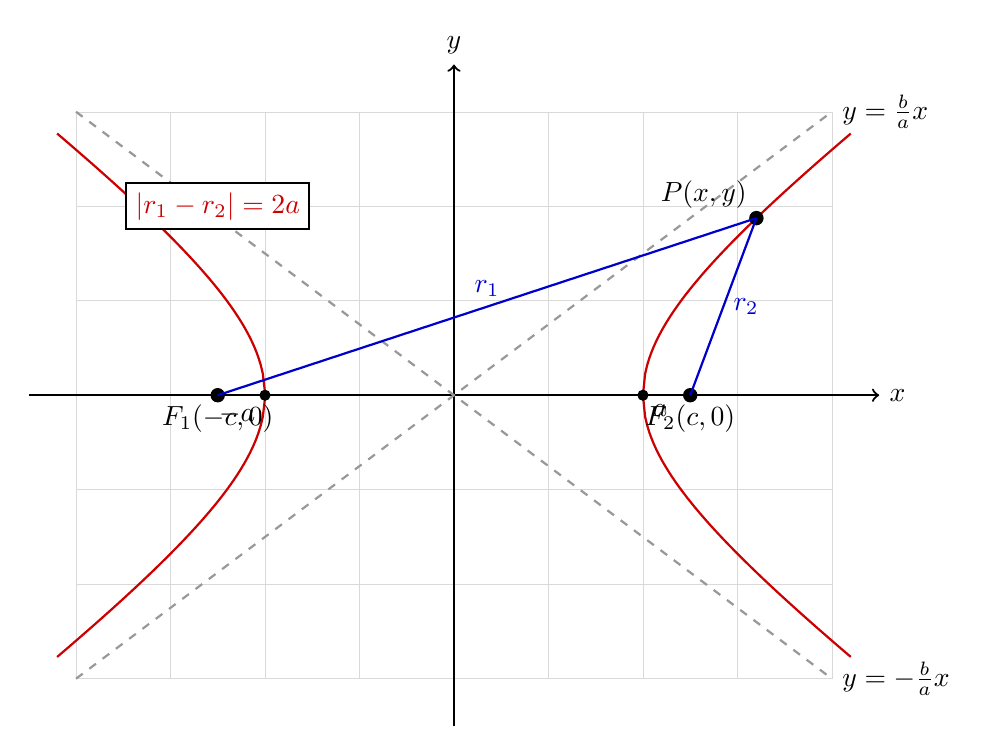
\begin{tikzpicture}[scale=1.2]
    % Rács és tengelyek
    \draw[step=1cm,gray!30,very thin] (-4,-3) grid (4,3);
    \draw[->,thick] (-4.5,0) -- (4.5,0) node[right] {$x$};
    \draw[->,thick] (0,-3.5) -- (0,3.5) node[above] {$y$};
    
    % Aszimptoták (y = +- (b/a)*x, ahol a=2, b=1.5 -> y = +- 0.75x)
    \draw[dashed, gray!80, thick] (-4, -3) -- (4, 3) node[right, text=black] {$y = \frac{b}{a}x$};
    \draw[dashed, gray!80, thick] (-4, 3) -- (4, -3) node[right, text=black] {$y = -\frac{b}{a}x$};
    
    % Hiperbola ágak rajzolása (a=2, b=1.5)
    % Jobb ág: felső és alsó rész
    \draw[bvred, thick, domain=2:4.2, samples=100] plot (\x, {1.5*sqrt((\x/2)^2 - 1)});
    \draw[bvred, thick, domain=2:4.2, samples=100] plot (\x, {-1.5*sqrt((\x/2)^2 - 1)});
    % Bal ág: felső és alsó rész
    \draw[bvred, thick, domain=-4.2:-2, samples=100] plot (\x, {1.5*sqrt((\x/2)^2 - 1)});
    \draw[bvred, thick, domain=-4.2:-2, samples=100] plot (\x, {-1.5*sqrt((\x/2)^2 - 1)});
    
    % Fókuszpontok c = sqrt(a^2 + b^2) = sqrt(4 + 2.25) = sqrt(6.25) = 2.5
    \coordinate (F1) at (-2.5, 0);
    \coordinate (F2) at (2.5, 0);
    \filldraw[black] (F1) circle (2pt) node[below] {$F_1(-c,0)$};
    \filldraw[black] (F2) circle (2pt) node[below] {$F_2(c,0)$};
    
    % Csúcspontok
    \filldraw[black] (2,0) circle (1.5pt) node[below right] {$a$};
    \filldraw[black] (-2,0) circle (1.5pt) node[below left] {$-a$};
    
    % Tetszőleges P pont és fókuszsugár távolságok
    \coordinate (P) at (3.2, 1.874); % Egy pont a jobb felső ágon
    \filldraw[black] (P) circle (2pt) node[above left] {$P(x,y)$};
    
    \draw[thick, blue!80!black] (F1) -- (P) node[midway, above] {$r_1$};
    \draw[thick, blue!80!black] (F2) -- (P) node[midway, right] {$r_2$};
    
    % Képlet kiírása a sarokba
    \node[draw, fill=white, thick, align=center] at (-2.5, 2) {\textbfr{$|r_1 - r_2| = 2a$}};
\end{tikzpicture}
\end{center}

\subsection*{Példák a hiperbola alkalmazására}
\begin{itemize}
    \item \textbf{Rutherford-kísérlet (Fizika):} Amikor pozitív töltésű alfa-részecskéket lőnek egy vékony aranyfóliára, az atommaggal való Coulomb-taszítás miatt a részecskék elhajlanak. A taszító centrális erőtérben a pályájuk egy hiperbolaág lesz.
    \item \textbf{Helymeghatározás (LORAN):} Két földi rádióadó azonos időben bocsát ki jeleket. A hajón lévő vevő méri a jelek beérkezése közötti időkülönbséget, ami megfelel a távolságok különbségének. A hajó lehetséges helyzete tehát egy hiperbola. Egy harmadik adóval metszéspontot, így pontos pozíciót kaphatunk.
\end{itemize}

\end{document}